\documentclass{article}

\usepackage{fullpage}
\usepackage{amsmath}
\usepackage{amsthm}
\usepackage{graphics}
\usepackage{graphicx}

\newtheorem{theorem}{Theorem}

\author{Olivier Beaumont, Lionel Eyraud-Dubois, Erik Saule}

\title{Fun with recursivity and parallel graph construction}

\begin{document}

\maketitle

\section{Multiplying Large Integers}

With $I_1 = aM + b$ and $I_2 = cM + d$ with $a,b,c,d < M$. Assume that
$I_1, I-2$ are of similar length which is $2^k$ words. $M$ is the
basis that maps to $2^{k-1}$ words.

\subsection{Variants}

\subsubsection{Naive}

The naive algorithm taught in elementary school is to compute:

\begin{align}
  I_1 * I_2 & = & a*c M^2 + (a * d + b * c ) M + b*d \\
            & = & (a*c)_{u} M^3 + ((a*c)_{l} + (a * d + b * c )_{u}) M^2 + ( (a * d + b * c )_{l} + (b*d)_{u} ) M + (b*d)_{l}
\end{align}

where the $x_u$ stands for the MSBs of $x$ and $x_l$ stand for the
LSBs of $x$. Indeed when multiplying $a*c$ (for instance), the result
can be almost as large as $M^2$ and therefore can are typically split
in two halves. (Note that there is a carry that bit that is ignored
here.)

\subsubsection{Karatsuba}

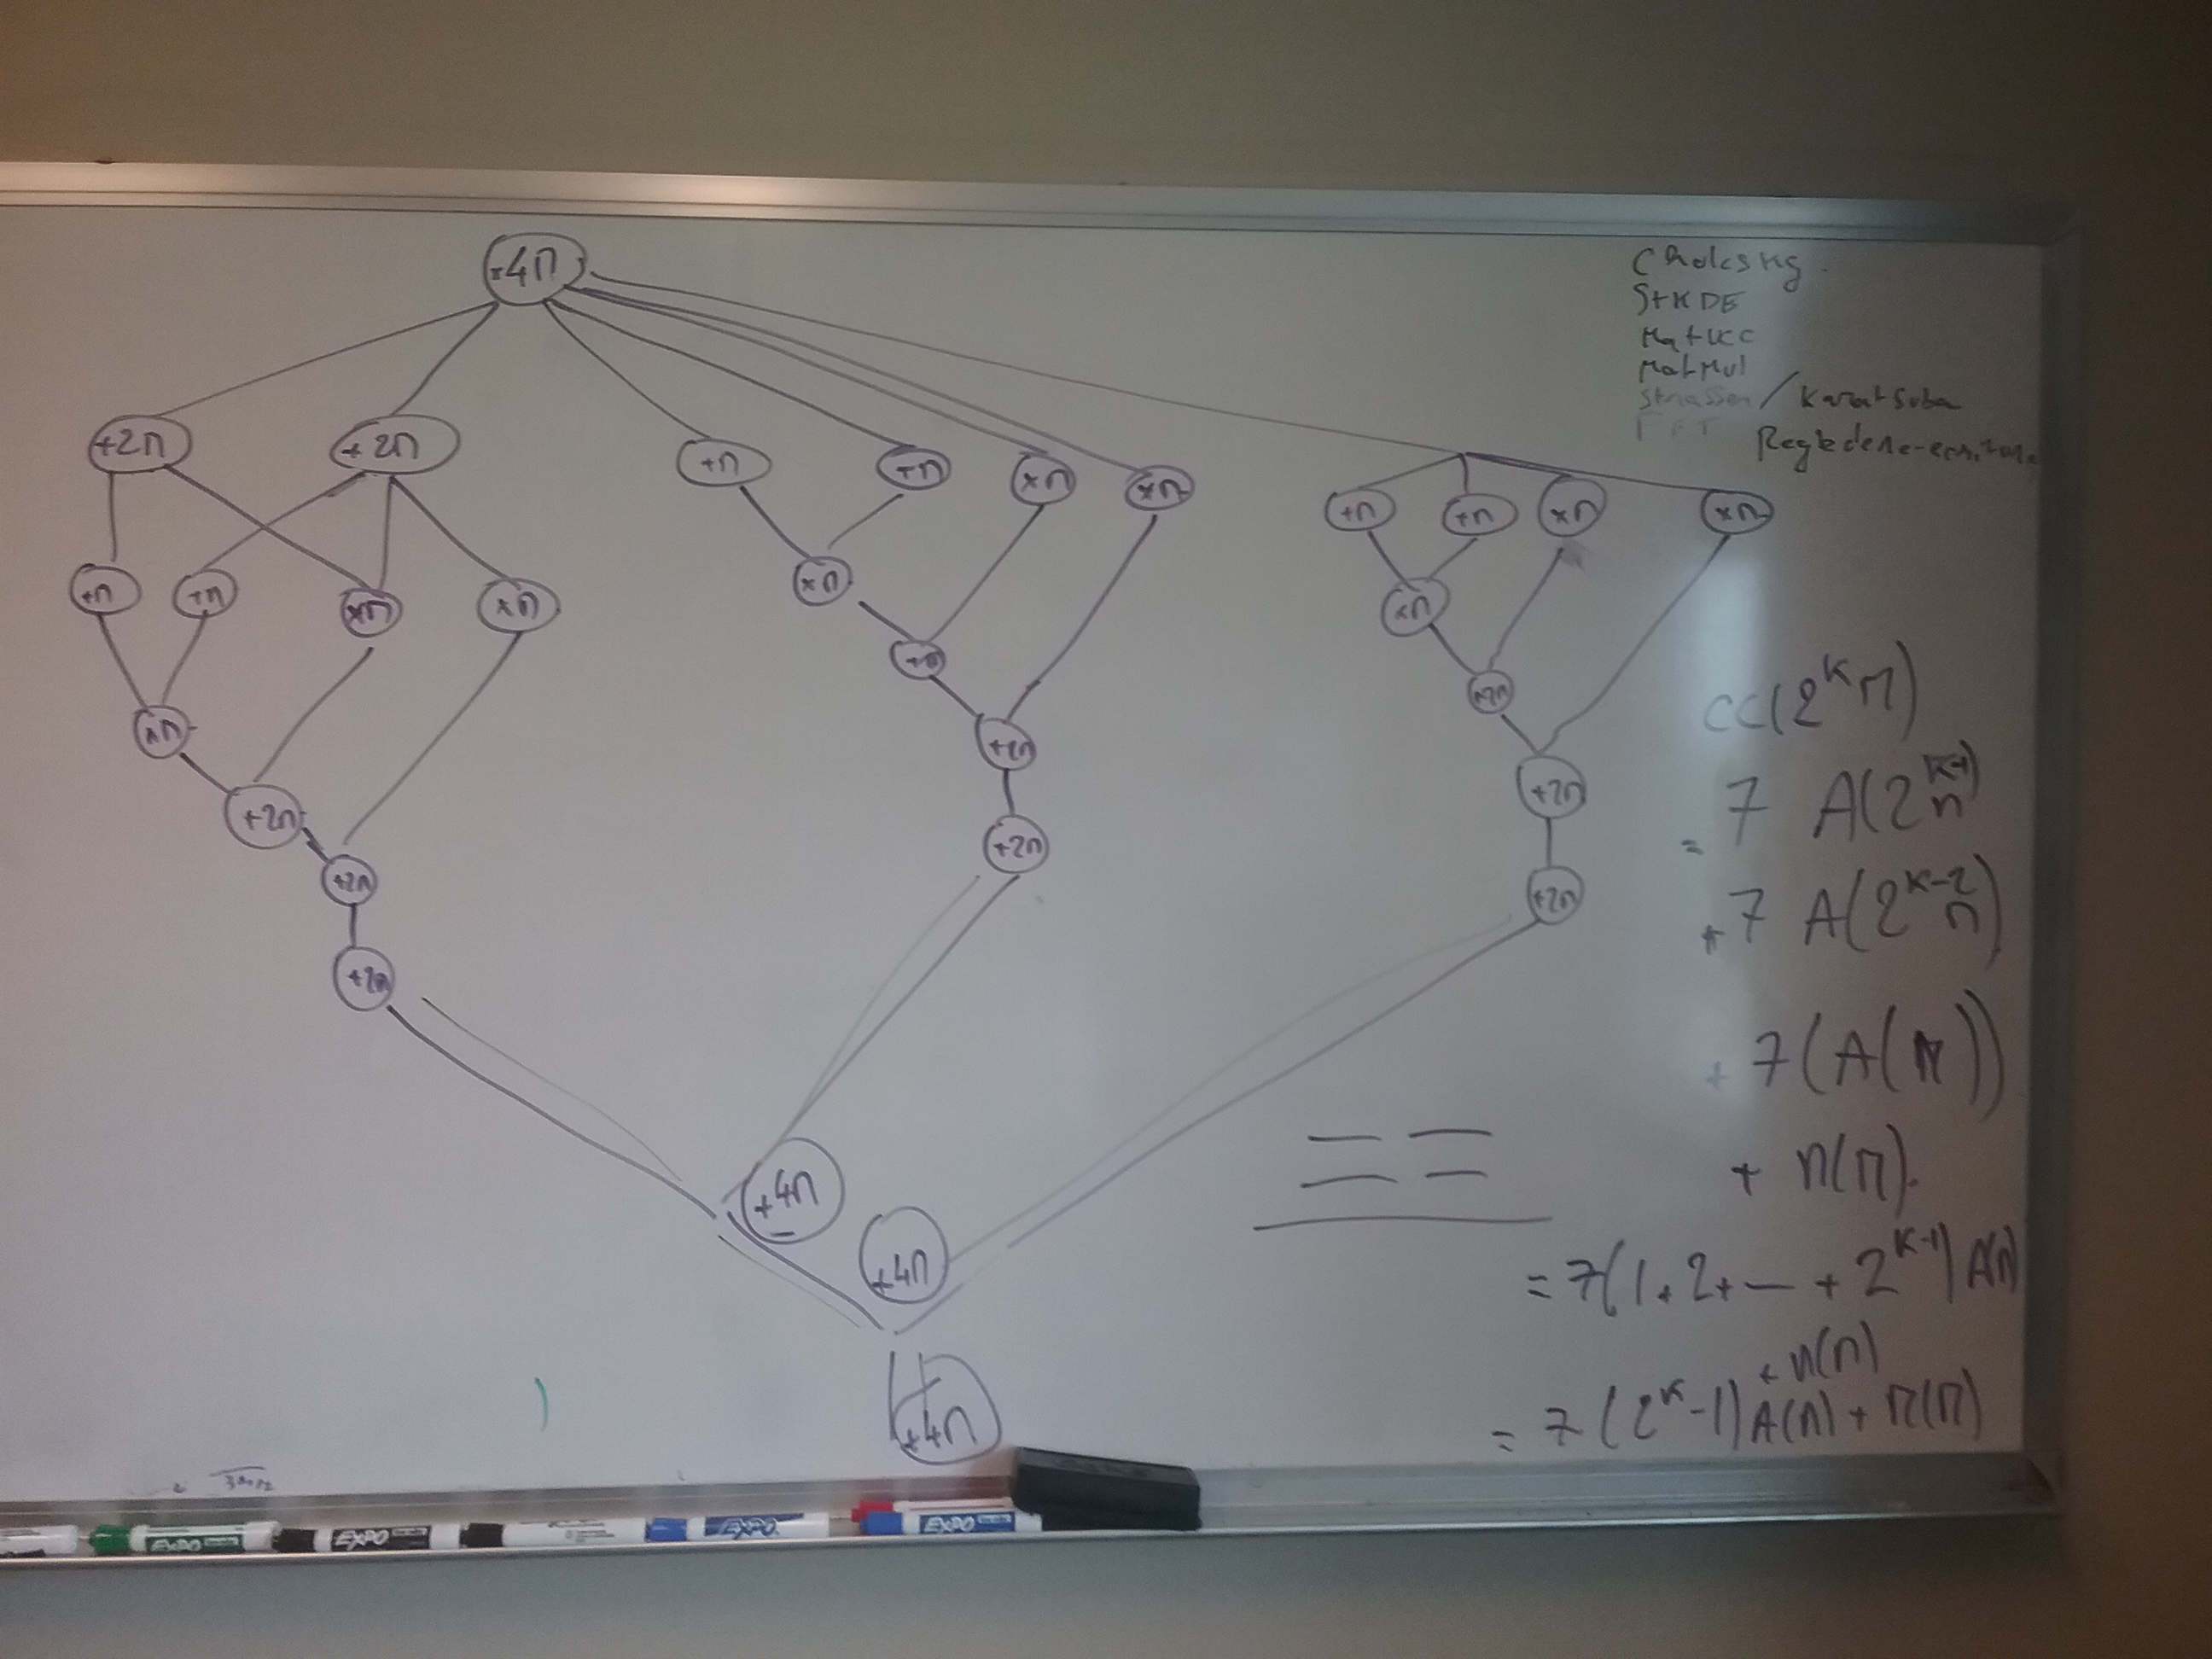
\includegraphics[width=.5\linewidth]{../../notes/20180608_120848.jpg}

\subsection{Hybridization}

\begin{theorem}
Karatsuba at high levels, naive then
\end{theorem}

\begin{proof}
\end{proof}

Analysis: 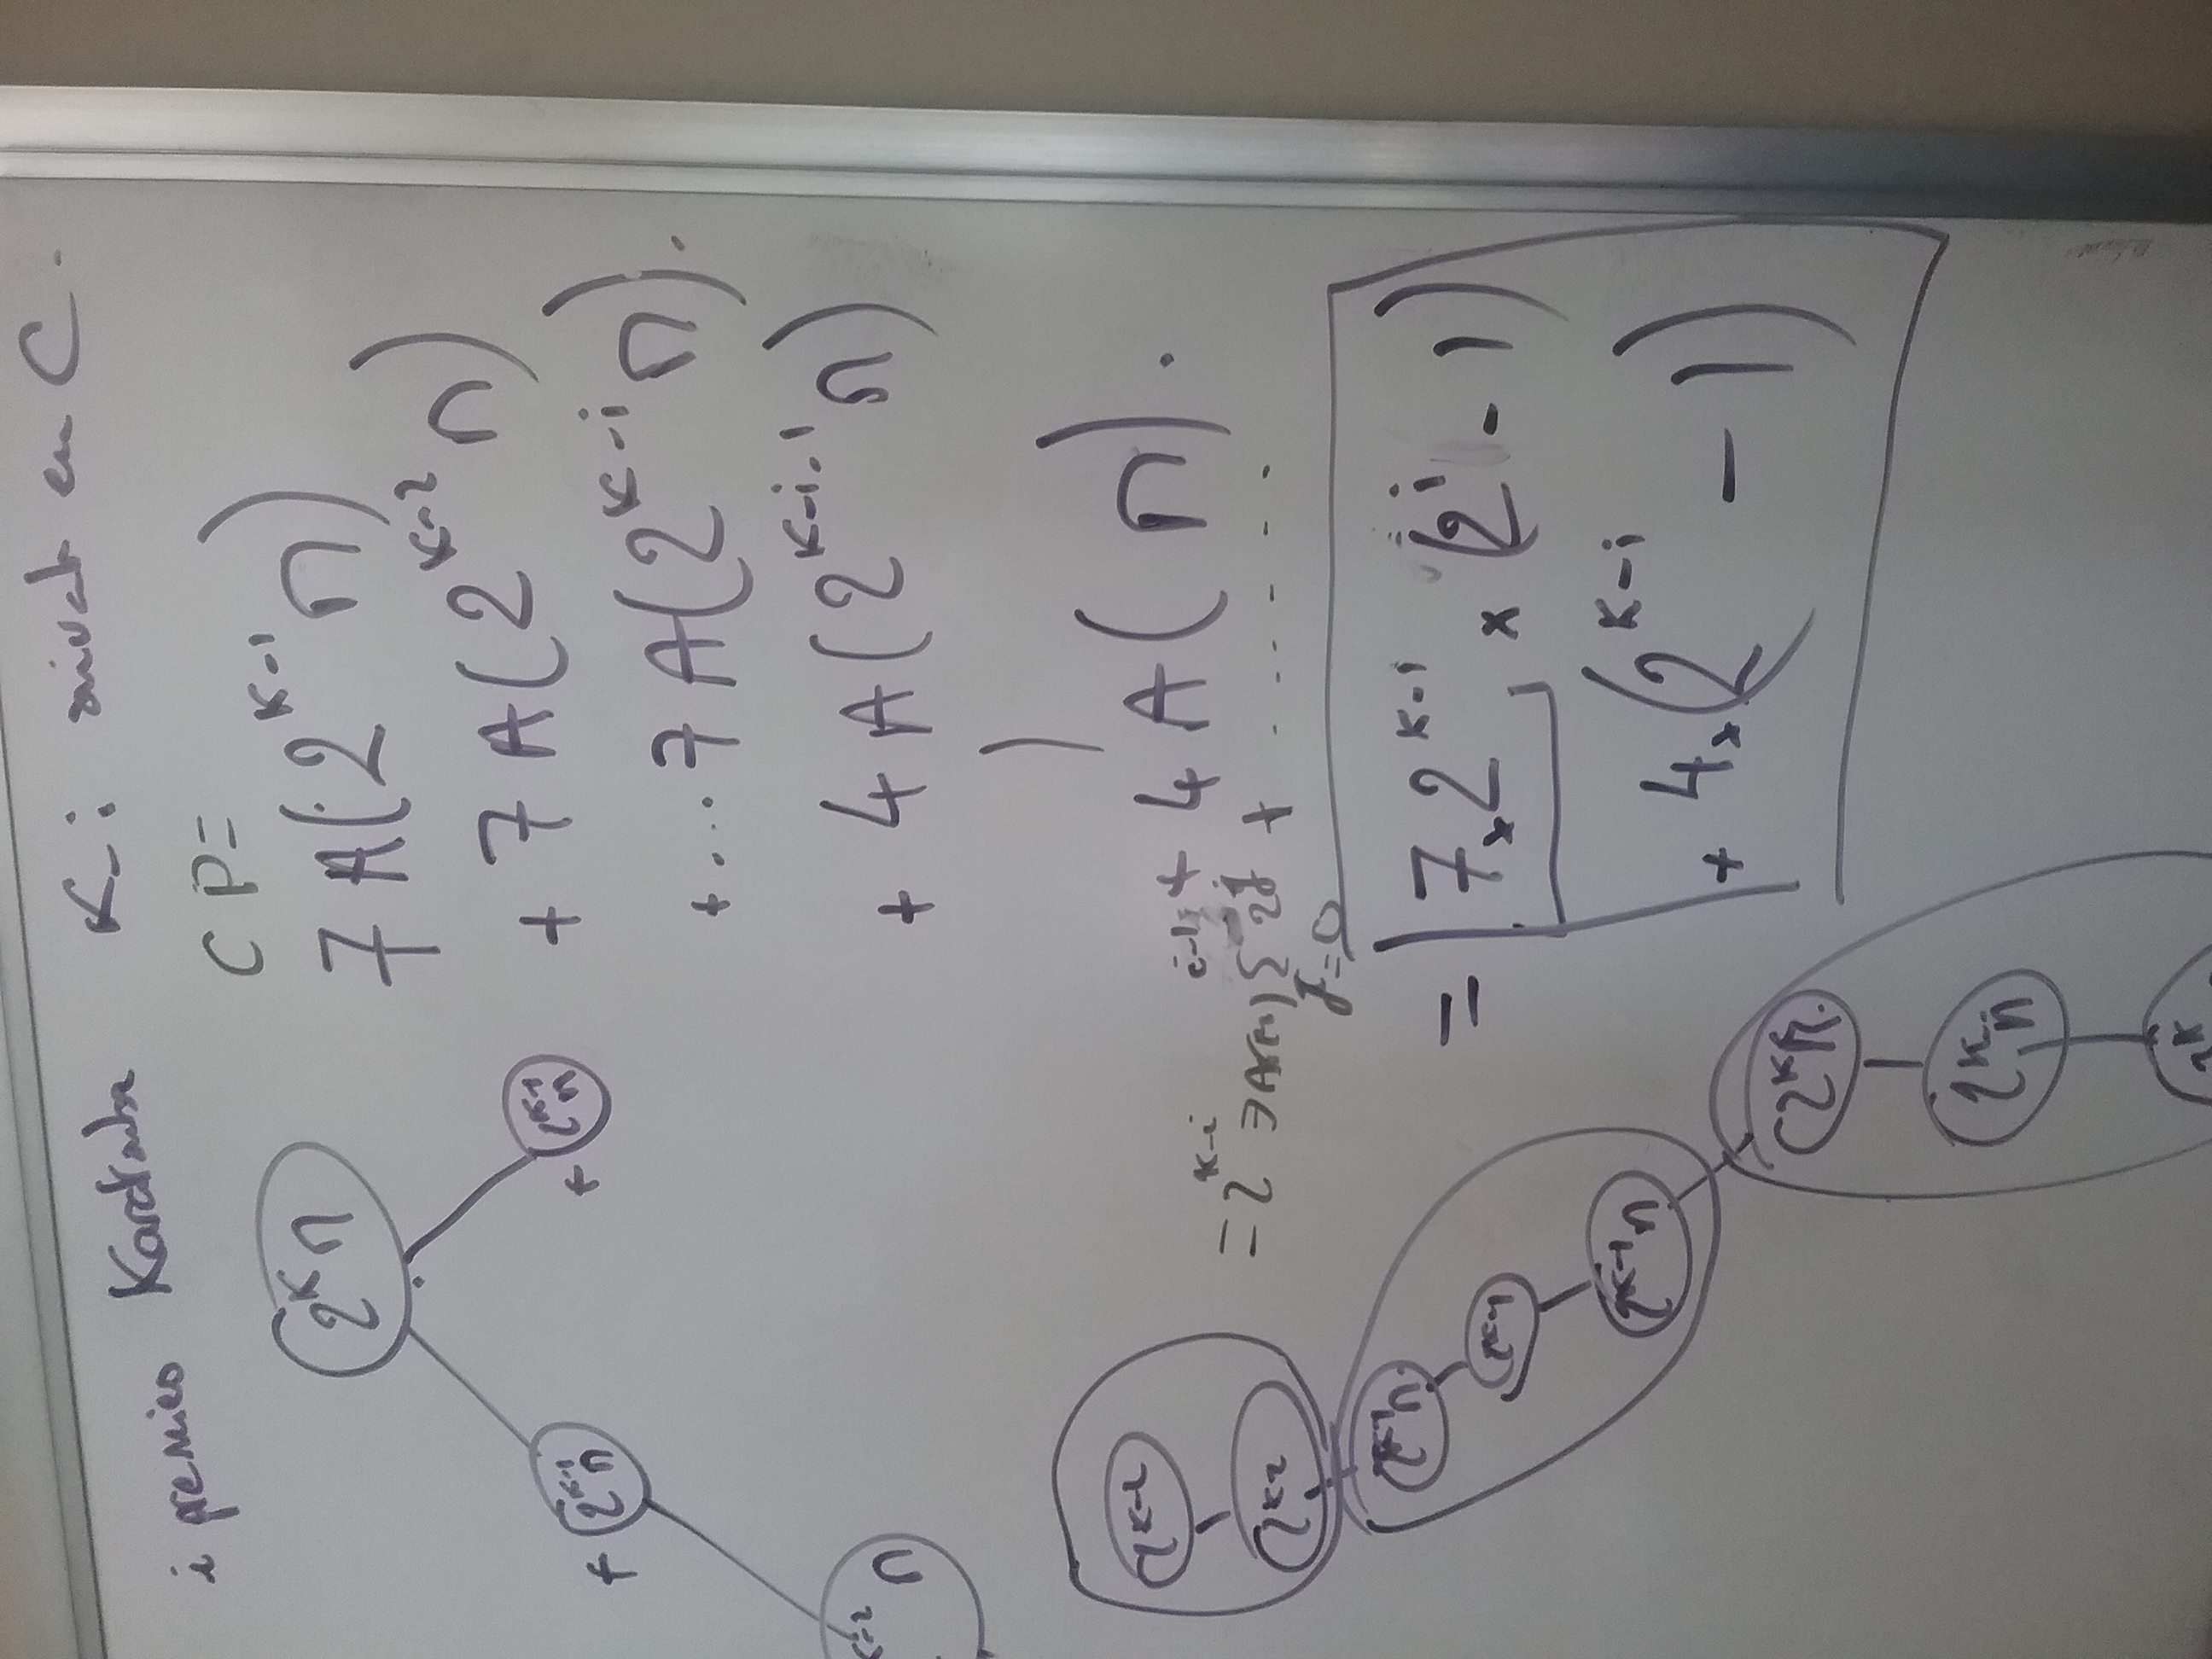
\includegraphics[width=.5\linewidth]{../../notes/20180608_142908.jpg}

\subsection{Generalization}

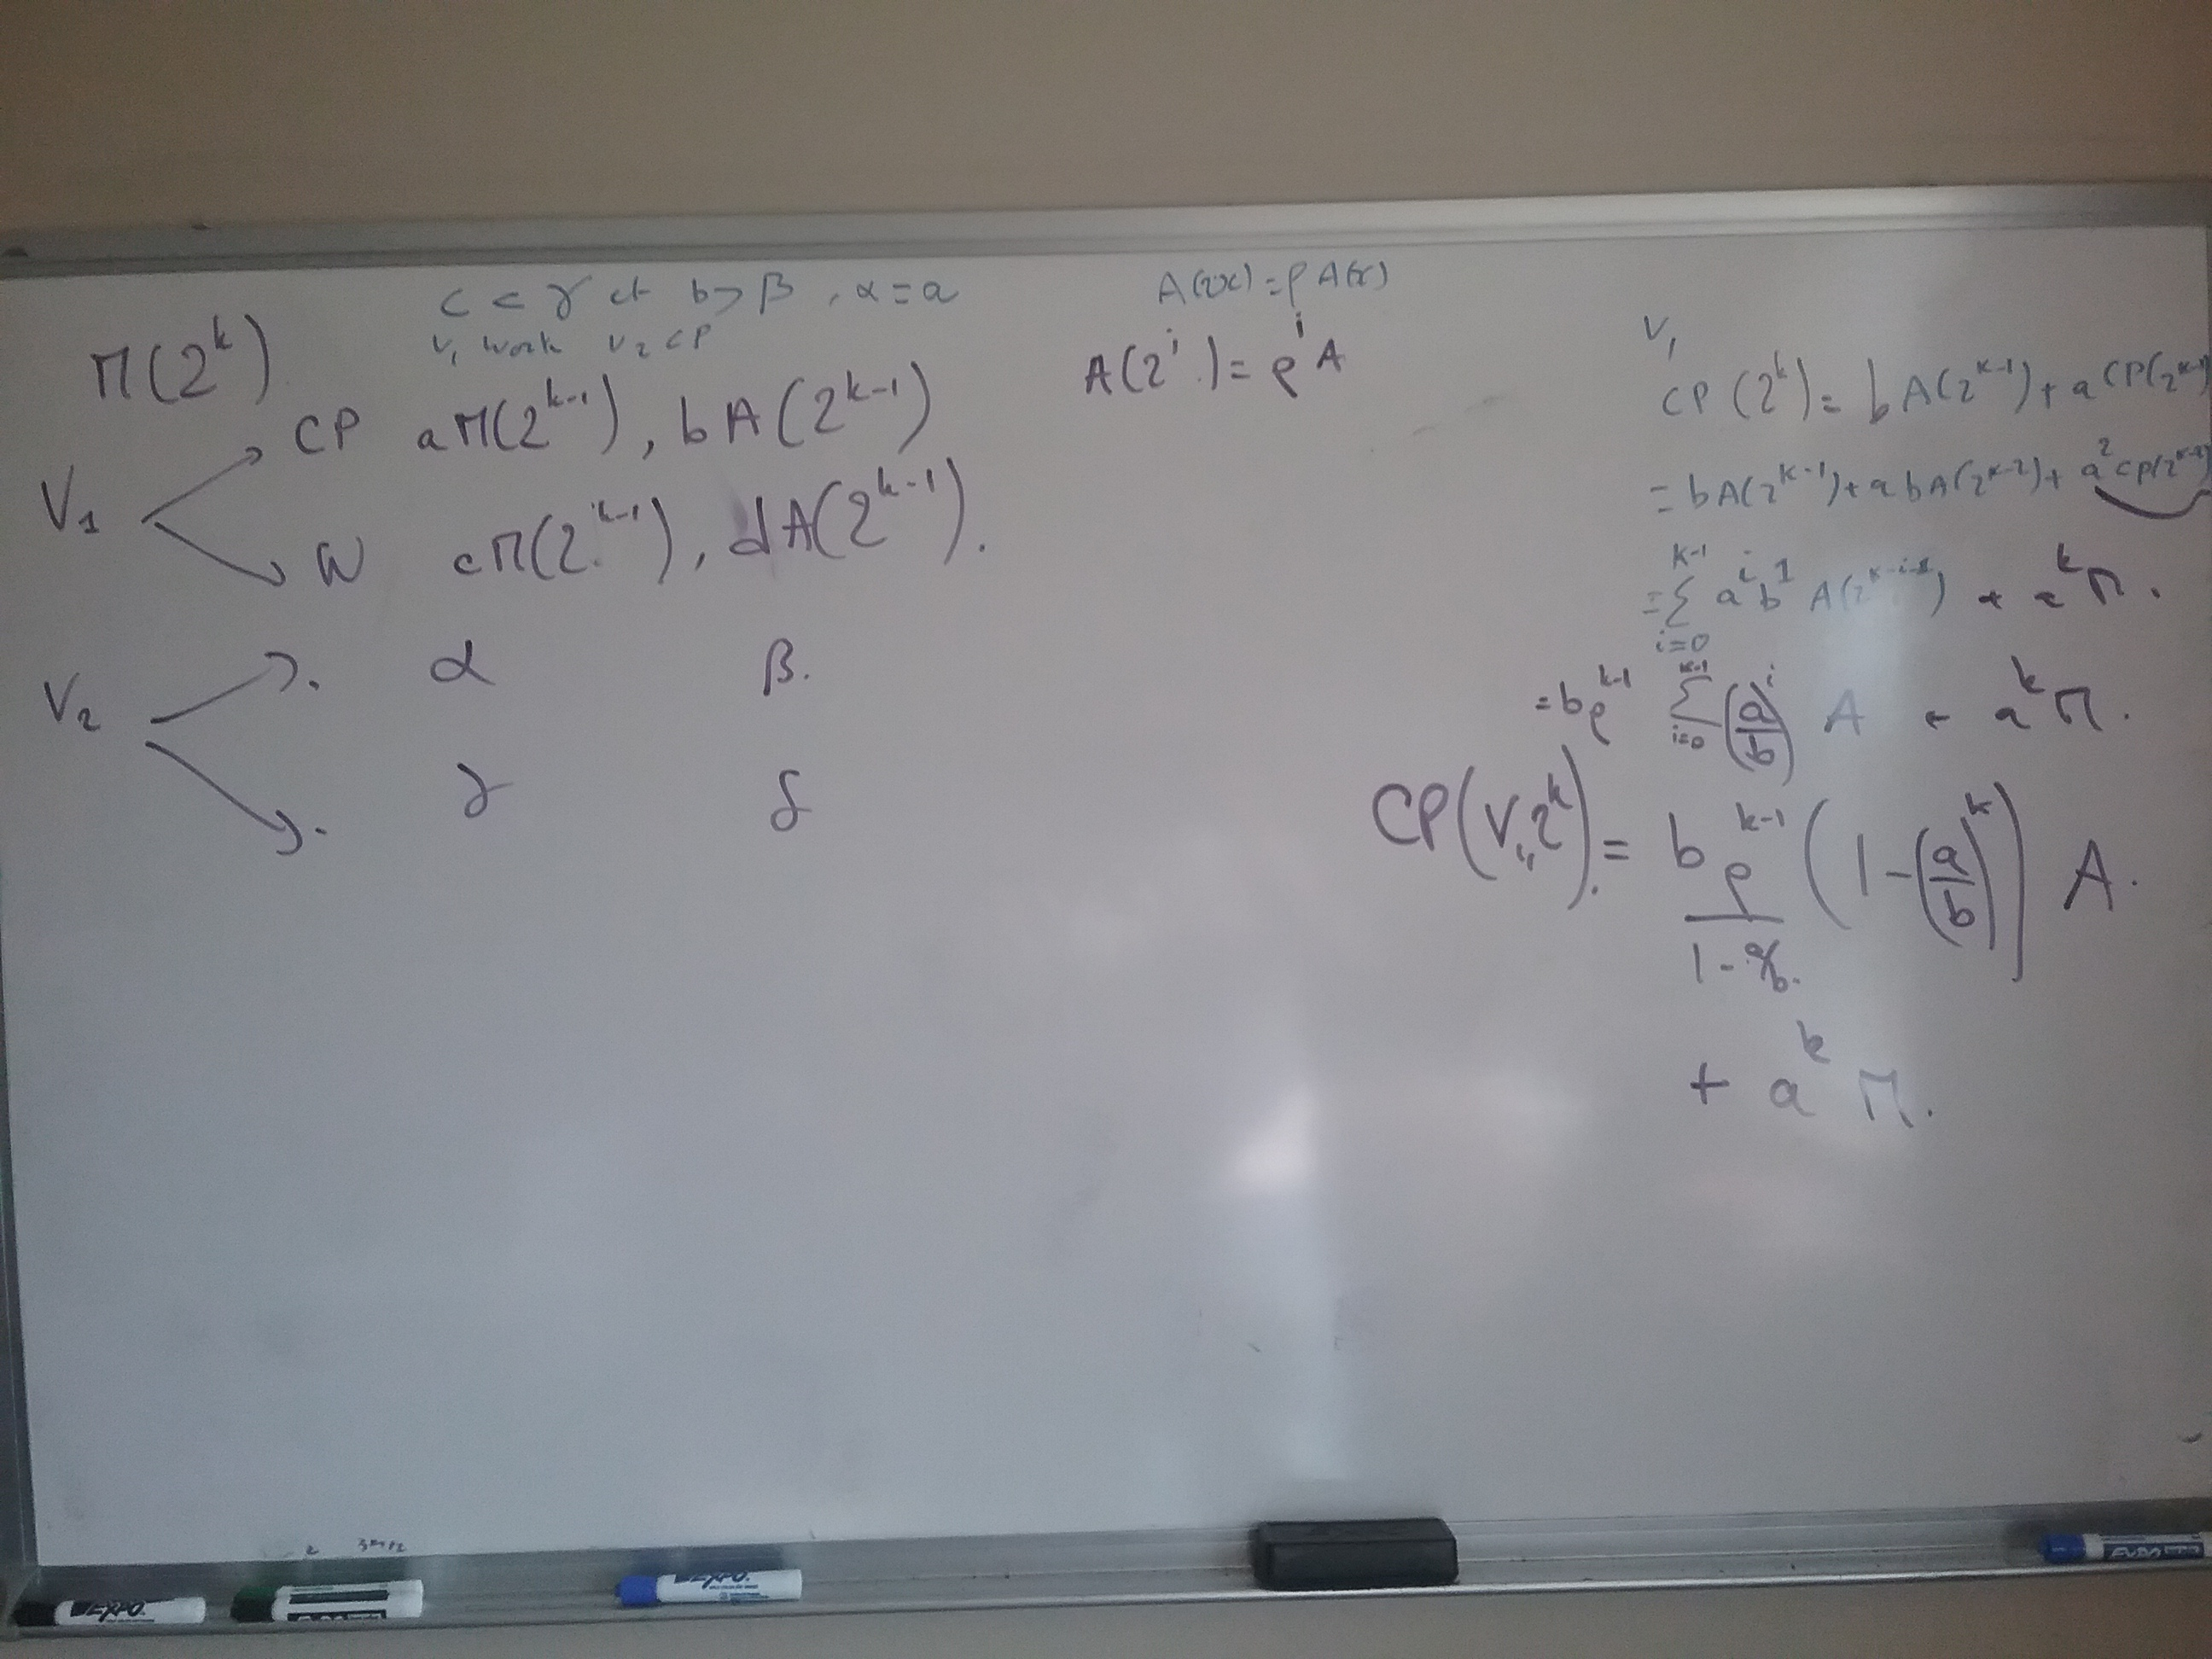
\includegraphics[width=.5\linewidth]{../../notes/20180608_172003.jpg}

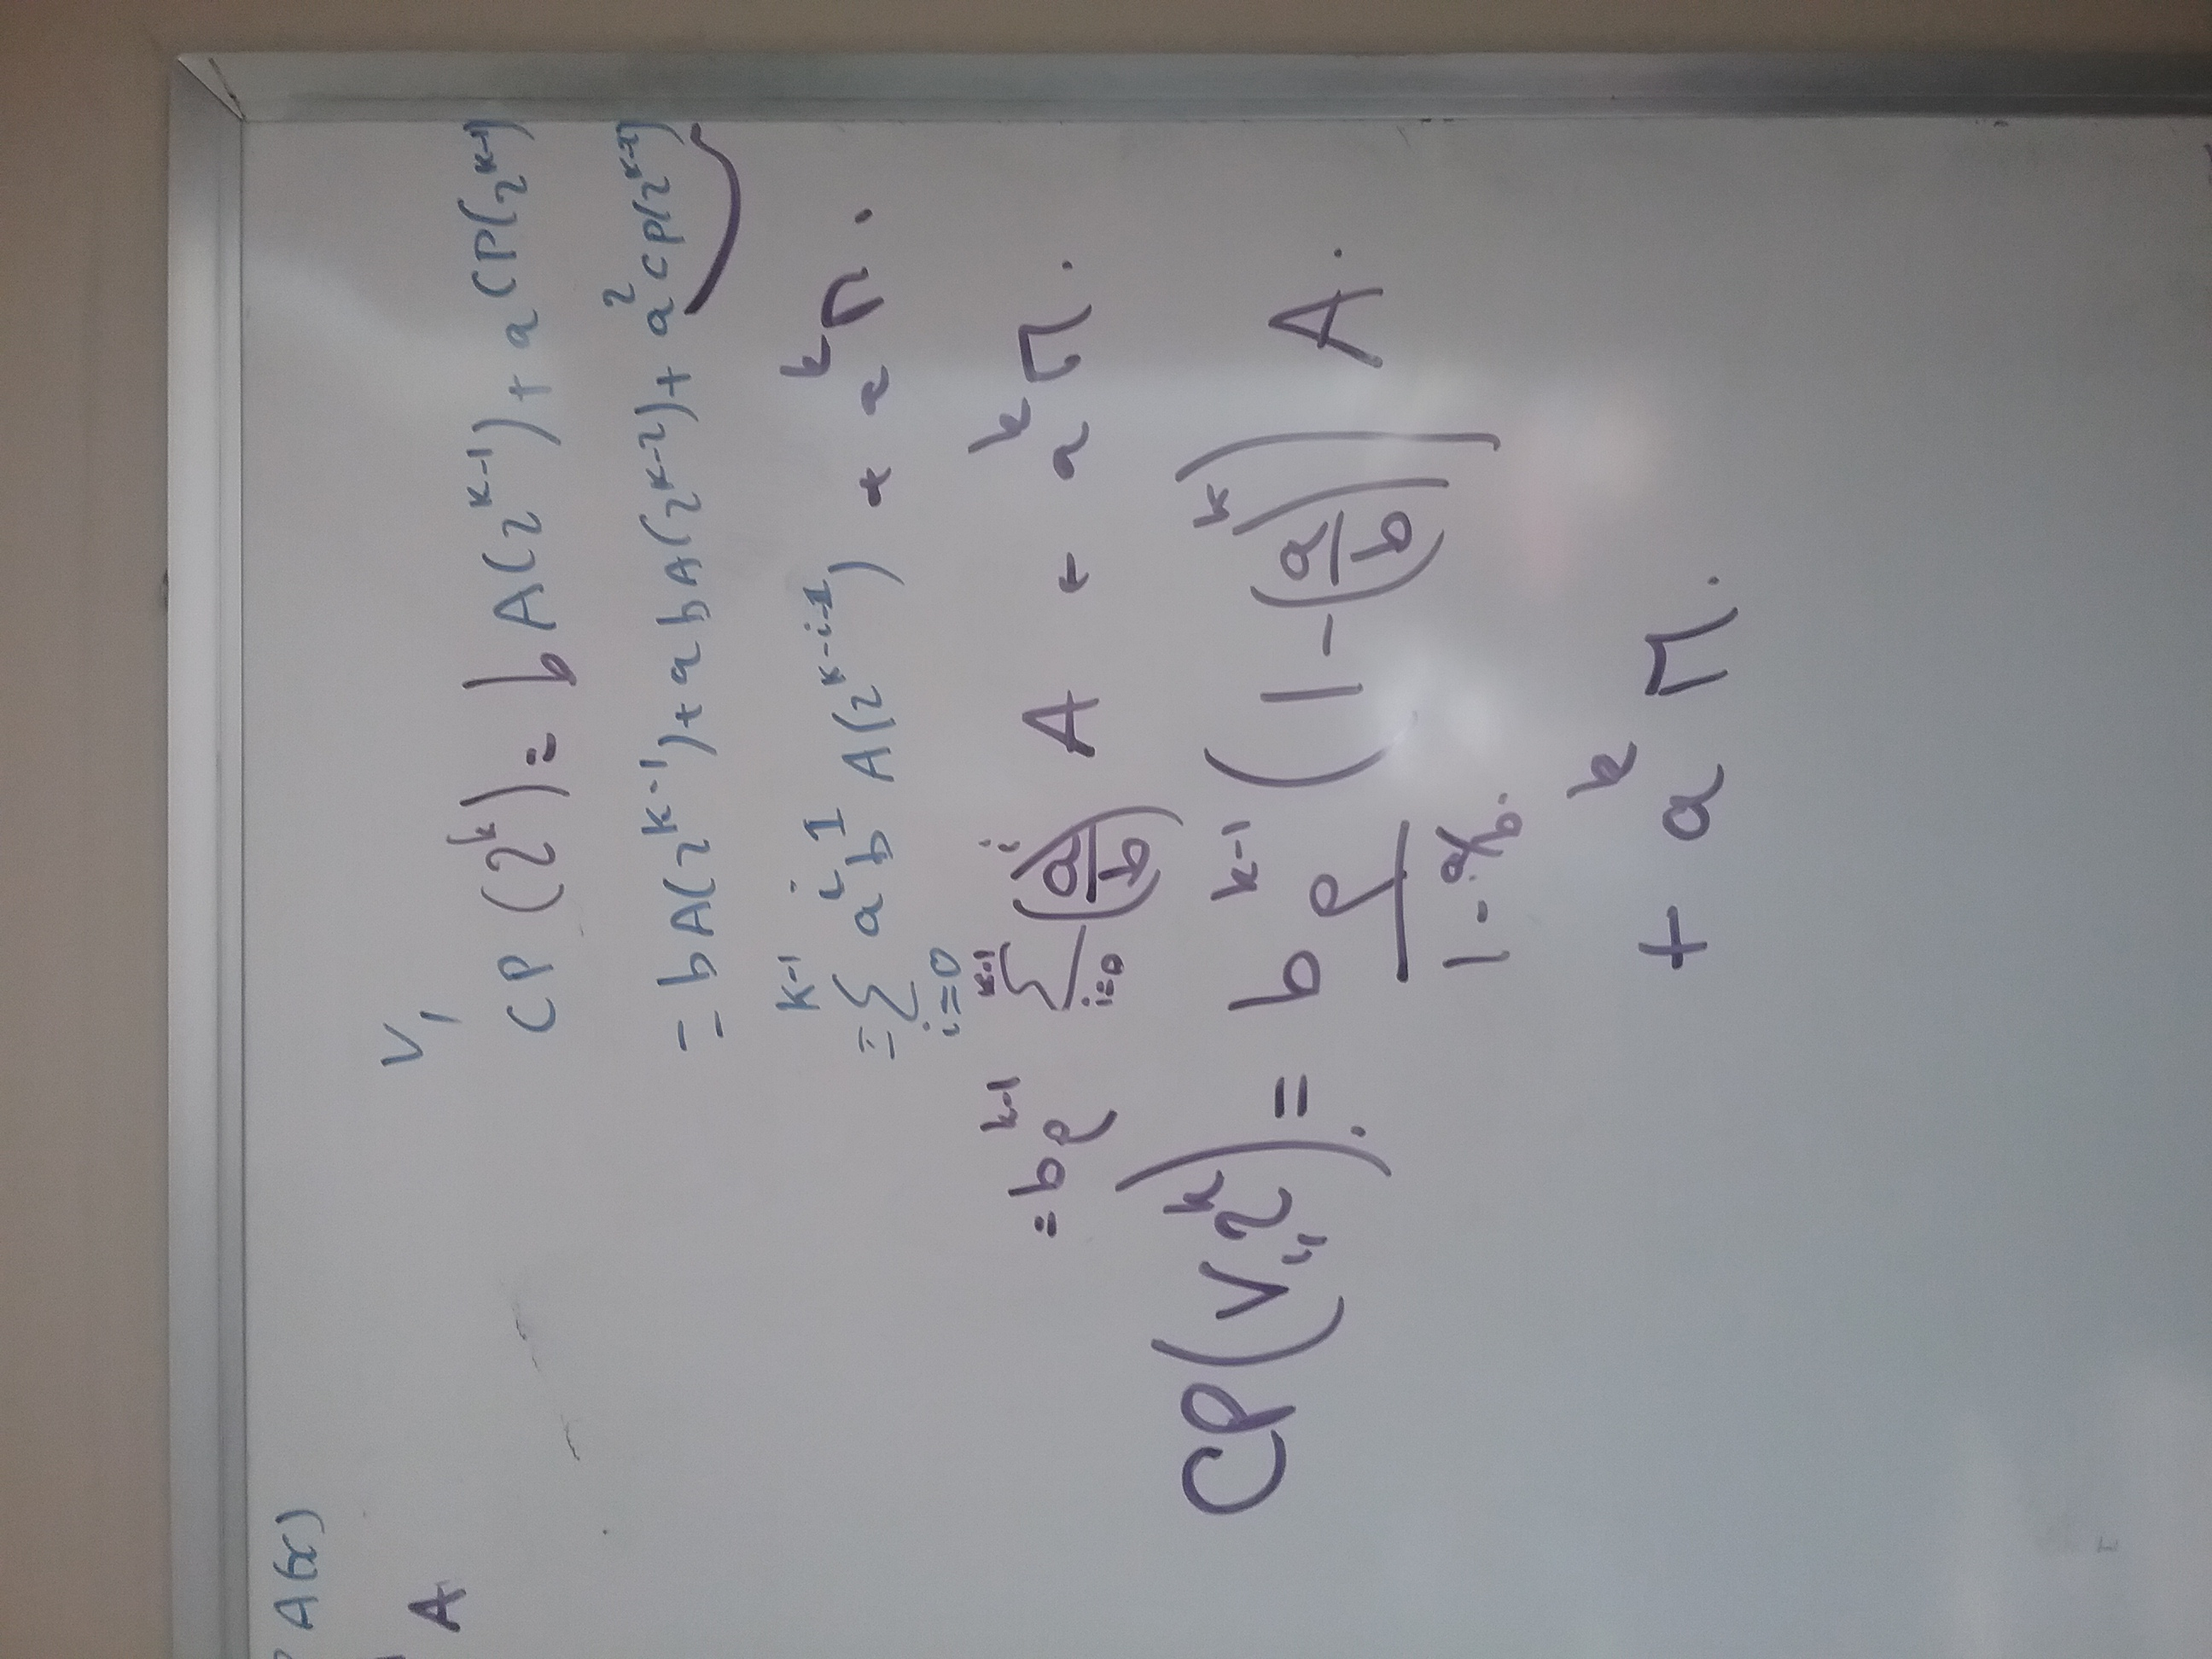
\includegraphics[width=.5\linewidth]{../../notes/20180608_172007.jpg}

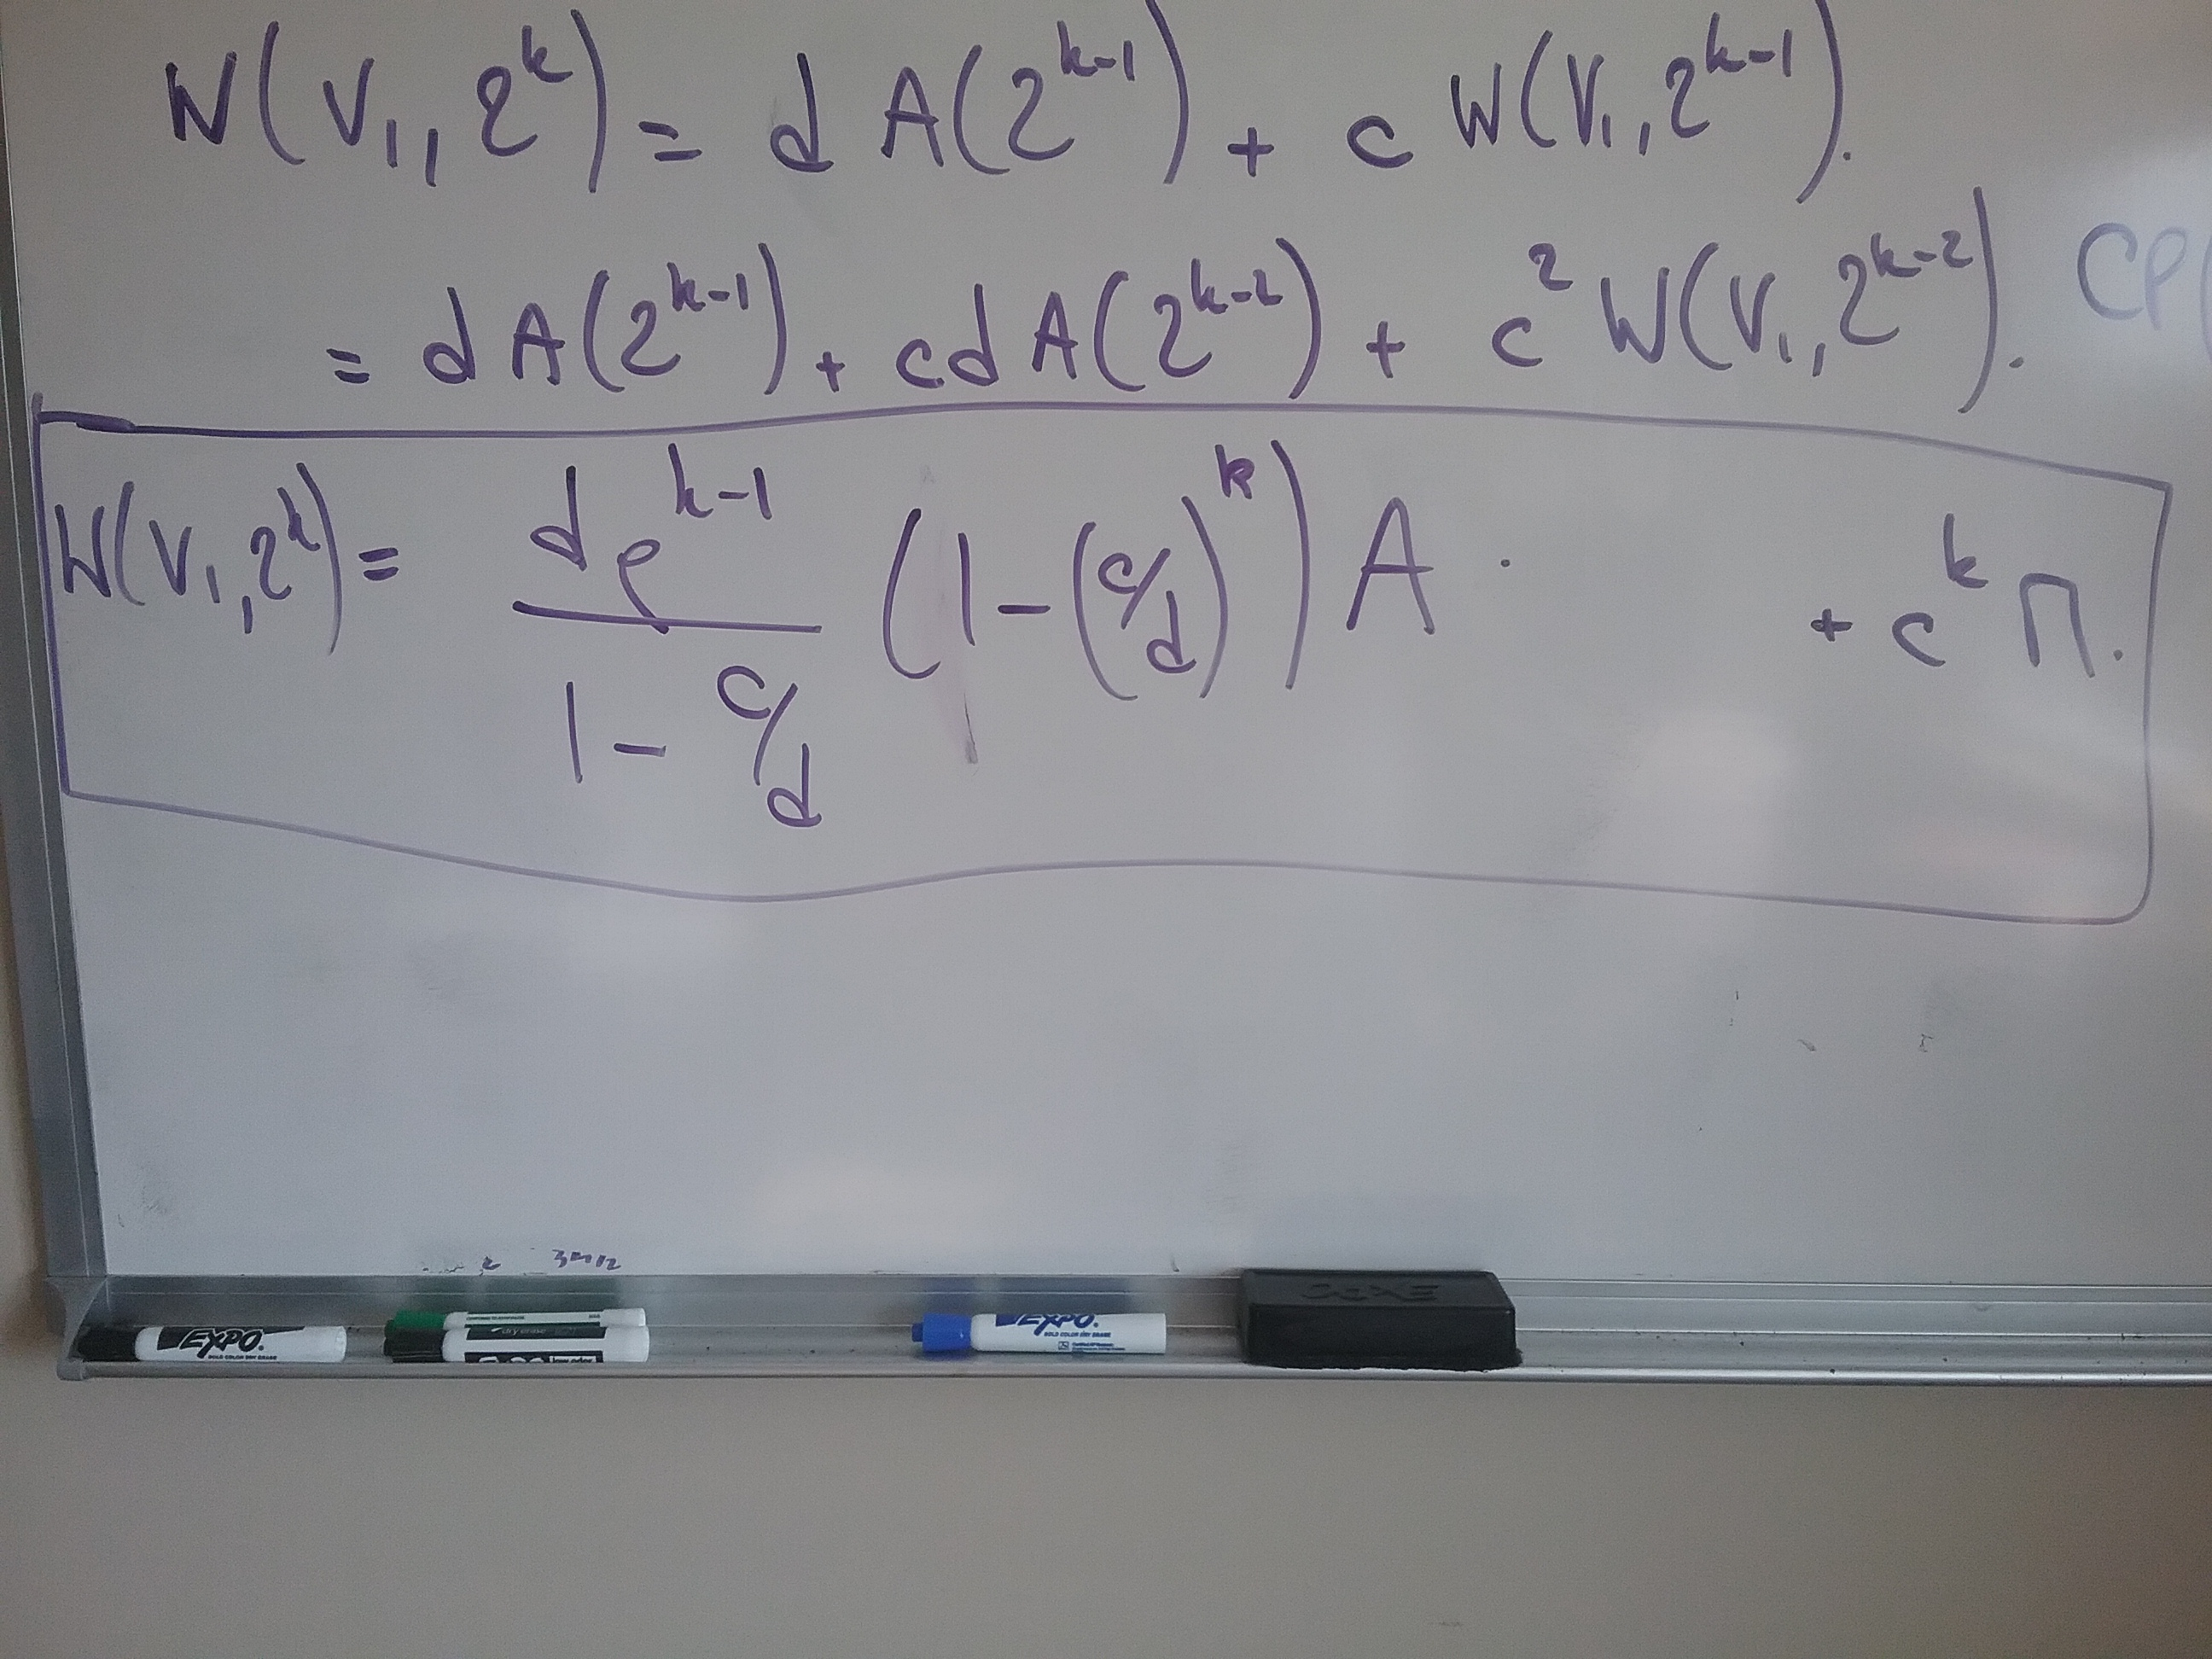
\includegraphics[width=.5\linewidth]{../../notes/20180608_172400.jpg}

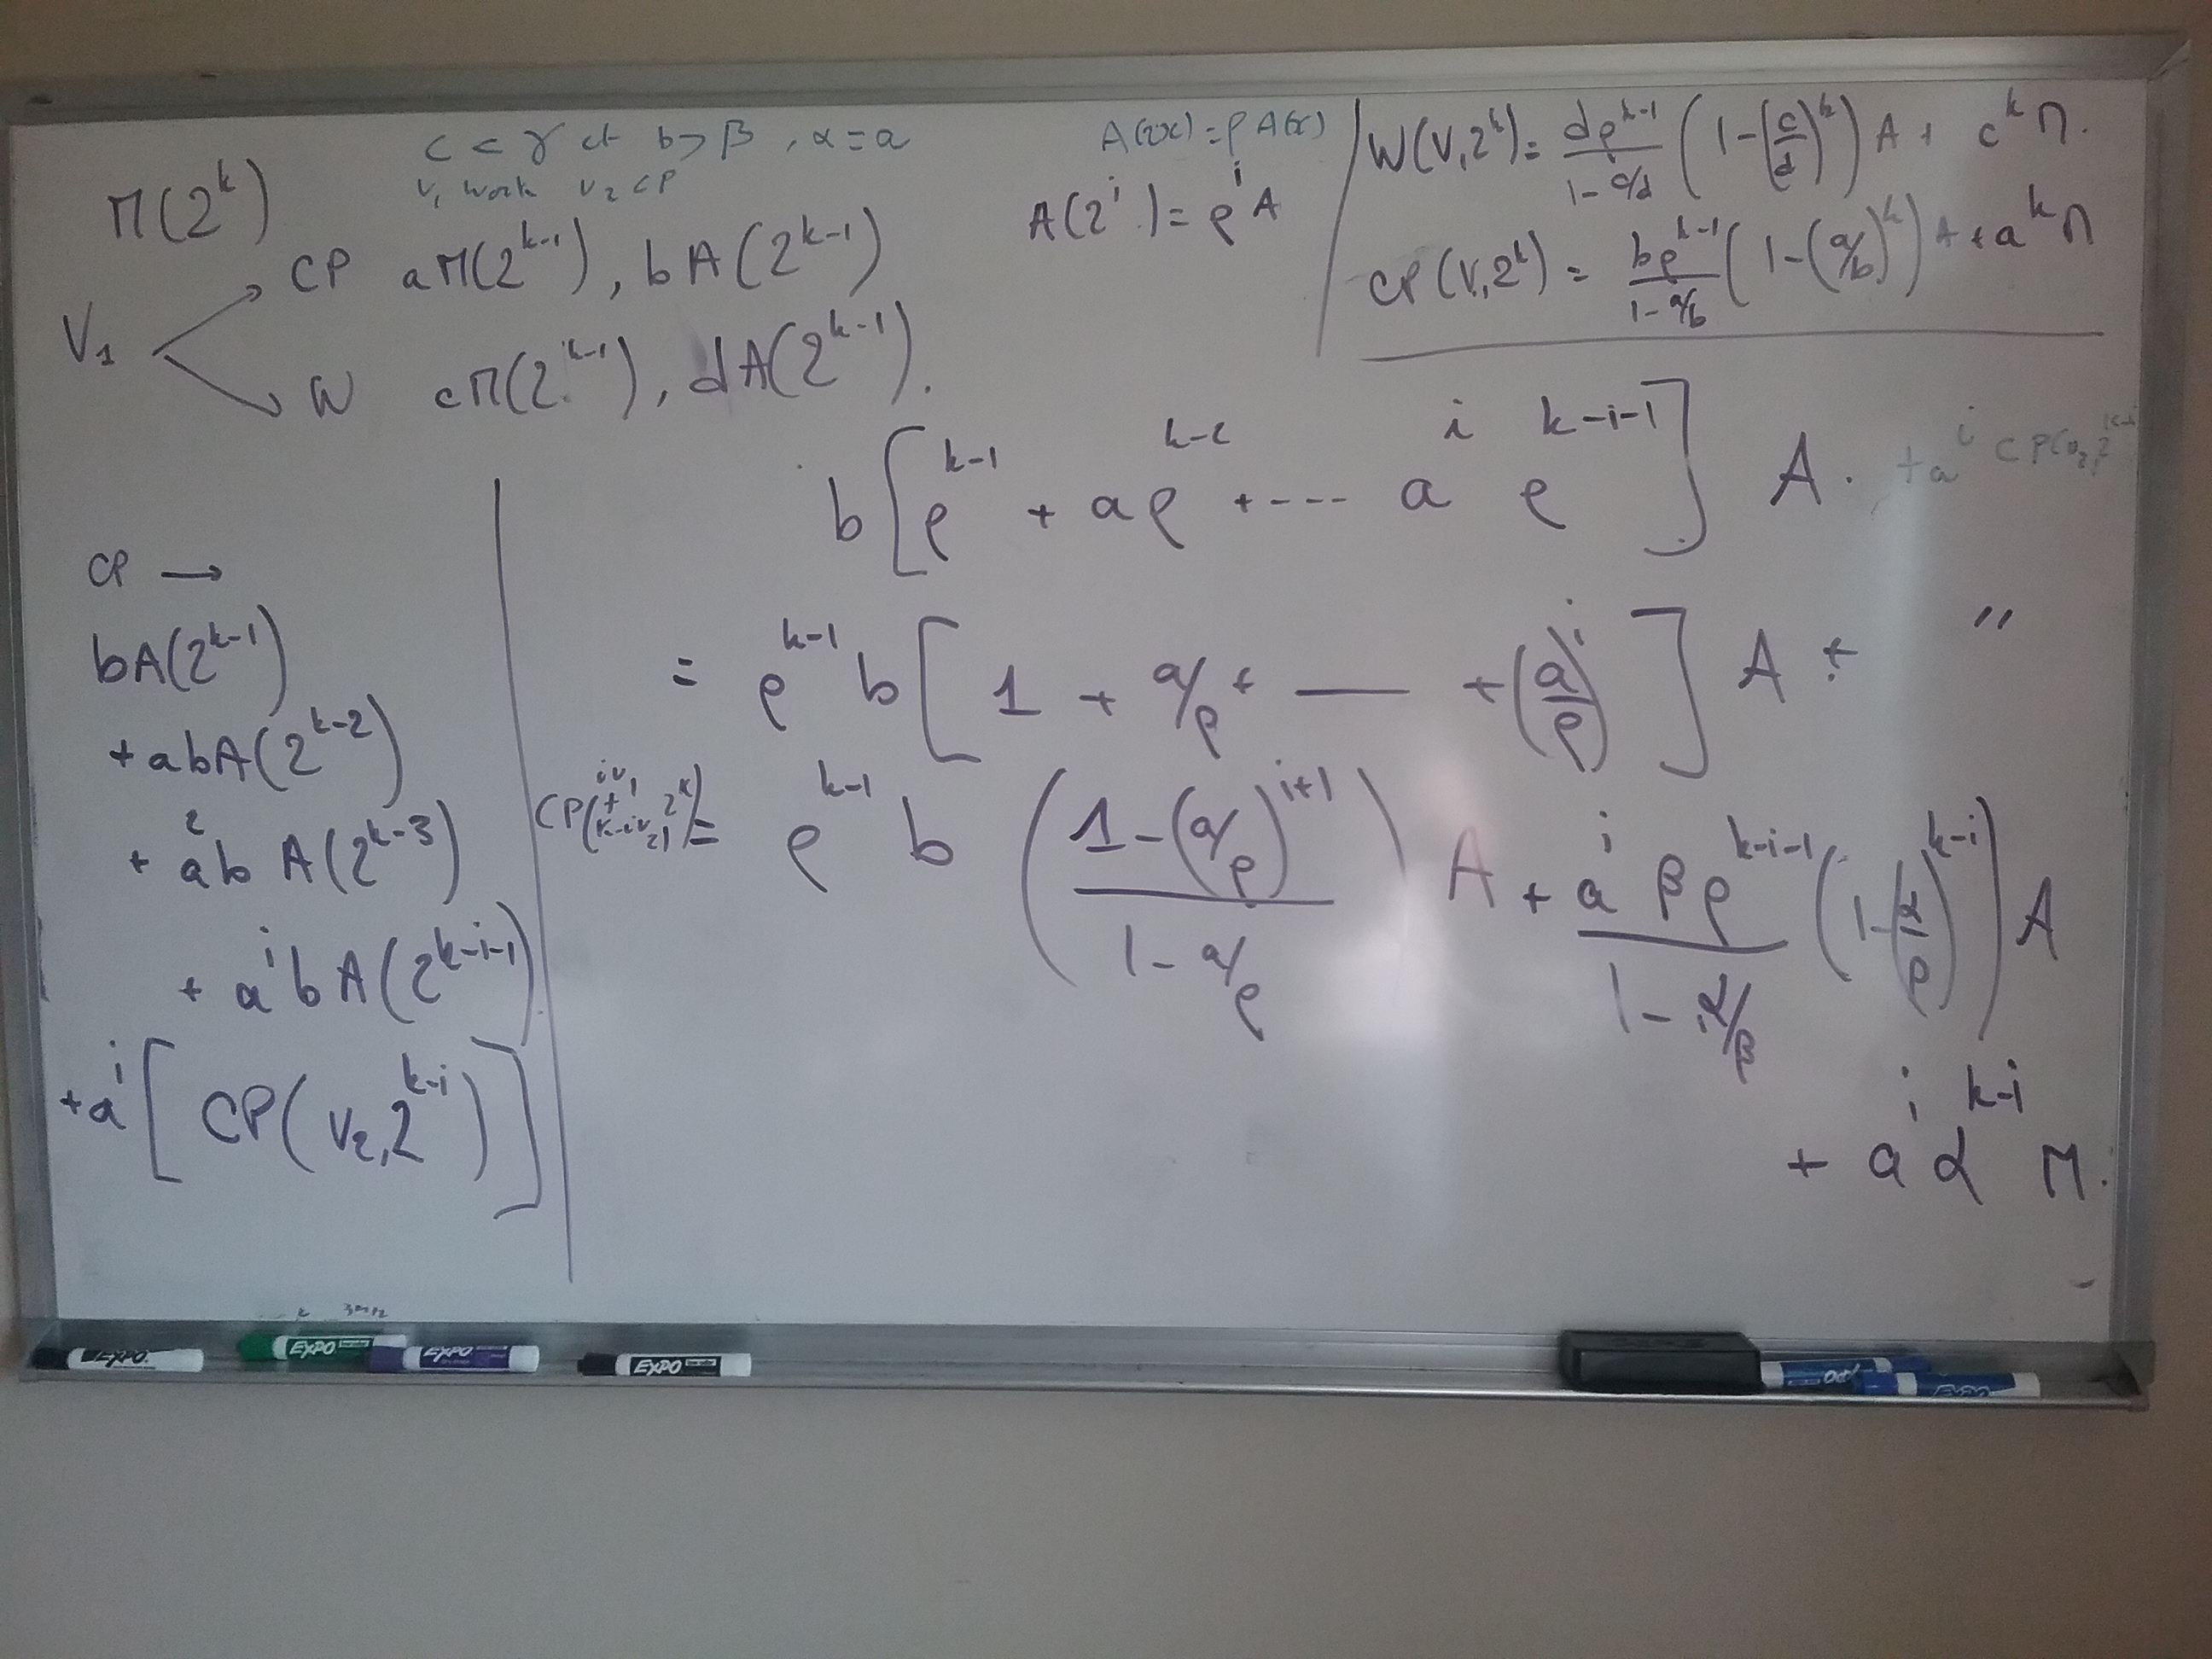
\includegraphics[width=.5\linewidth]{../../notes/20180608_175854.jpg}

\section{MergeSort}

\subsection{Variants}

\subsubsection{Sequential Merge}

With sequential merge, we have an in-tree of merges with the root
being of $Merge(n)$, one level down being 2 $Merge(n)$, etc.

This leads to $Merge^W(n) = n$ and $Merge^{CP}(n)=n$. $MergeSort^W(n)
= n \log n$ and $MergeSort^{CP}(n) = 2n$.

\subsubsection{Parallel Merge}

Merge can be made parallel. When merging two arrays of size $n/2$. Cut
the first one in half and find the corresponding cut location in the
second array (using a binary search). To get good load balancem, one
needs to also cut the second array and find the corresponding location
in the first array, leading to 3 chunks that need to be cut.

One can assume that a single cut is enough for analysis purposes,
thought the more complex algorithm is necessary to reach the correct
bounds.

One can generalize that cut by having $P$ cuts, and performing P
binary searches on each side, there is a need to reconcile the cuts
position which cost a merge of size $2P$. This leads to $Merge^W(n,P) =
n + 2 P \log n + 2P$, the $n$ term is for all the merges, the $2P \log
n$ are for the binary search and the $2P$ is for the merge of size
$2P$. And $Merge^{CP}(n,P) = n/P + \log n + 2P$, the $n/P$ term
is for the final merge, the $\log n$ comes from the parallel binary
searches, and the $2P$ comes from the merge of size $2P$ in parallel.

Since obtaining more parallelism is a costly operation in term of
work, for ParallelMergeSort, the optimal solution is clearly to have
$P$ tasks for level 0, $P/2$ tasks for each merge at depth 1,
$P/4$ tasks for each merge at depth 2, ... Defaulting to sequential
merges at depth $\log P$

For this parallel merge sort, the work becomes
$ParallelMergeSort^W(n) = n \log n + 2 P \sum_{i=0}^{\log P - 1} \log n/2^i + 1$
since the term in $n$ does not change
from merge sort and the splitting overhead is of $2P (\log n/2^i + 1)$ at
level $i$. So
\begin{align}
  ParallelMergeSort^W(n) & = & n \log n + 2 P \sum_{i=0}^{\log P - 1}( \log n/2^i + 1  )\\
  & = &n \log n + 2 P \left (\log P (\log n +1)- \sum_{i=0}^{\log P - 1} \log 2^i  \right )  \\
  & = &n \log n + 2 P \left (\log P (\log n +1)- \sum_{i=0}^{\log P - 1} i \right )  \\
  & = &n \log n + 2 P \left ( \log P (\log n +1)- \frac{(\log P - 1)(\log P)}{2}   \right) \\
  & = &n \log n + 2 P \log P \left (  \log n + 1 - \frac{\log P - 1}{2}   \right)  
\end{align}

and the critical path becomes


\section{QuickSort}



\end{document}
